% Structure of the hierarchical model built in Model_B/Build_Model_B.py

\documentclass[11pt]{article}
\usepackage[margin=1in]{geometry}
\usepackage{amsmath,amssymb}
\usepackage{booktabs}
\usepackage{tikz}
\usetikzlibrary{positioning,fit,arrows.meta,calc}
\usepackage[hidelinks]{hyperref}

\newcommand{\invlogit}{\operatorname{logit}^{-1}}
\newcommand{\code}[1]{\texttt{#1}}

\title{Model B: Structure of the Hierarchical Psychometric Model}
\author{Vera Schroeder}
\date{October 1, 2026}

\begin{document}
\maketitle

\noindent
This document describes the model defined in \code{Model\_B/Build\_Model\_B.py}.
Model B fits a psychometric function with two asymptote (lapse) parameters to
every session of every group, and links the sessions of each group through
group-level hyperparameters.

%------------------------------------------------------------------------------
\section{Data and indexing}

The data are $N$ binary trials. Trial $i$ has
\begin{itemize}
  \item a response $y_i \in \{0,1\}$ (\code{obs\_data});
  \item a standardized stimulus amplitude $x_i$. The raw amplitudes are centred
        and scaled by the mean and standard deviation of the distinct amplitude
        levels (\code{DataProcessing\_B.py}). The covariate row is
        $(1, x_i)$ (\code{cov\_mat});
  \item a group $g[i] \in \{1,\dots,4\}$ (\code{grp\_idx}): the combination of
        hand and distractor condition,
        \[
          g \in \{\text{left\_uni},\ \text{left\_bi},\ \text{right\_uni},\ \text{right\_bi}\},
        \]
        where ``uni'' is unimanual (no distractor) and ``bi'' is bimanual
        (distractor present);
  \item a session $s[i] \in \{1,\dots,S\}$ (\code{sess\_idx}); the real data have
        $S = 42$.
\end{itemize}
Every combination of group $g$ and session $s$ has its own set of psychometric
parameters, so the model has $4S$ psychometric functions.

%------------------------------------------------------------------------------
\section{Likelihood}

Each response is Bernoulli,
\[
  y_i \sim \text{Bernoulli}(\psi_i), \qquad
  \psi_i = \psi\big(x_i;\ \theta_{g[i],s[i]}\big),
\]
with the psychometric function
\[
  \psi(x;\theta) = \gamma_h + (1 - \gamma_h - \gamma_l)\,\invlogit(b_0 + b_1 x),
  \qquad \theta = (b_0, b_1, \gamma_h, \gamma_l).
\]
Here $b_0$ is the bias (intercept), $b_1$ the slope, and $\gamma_h,\gamma_l$
set the asymptotes:
\[
  \lim_{x\to-\infty}\psi = \gamma_h, \qquad \lim_{x\to+\infty}\psi = 1-\gamma_l .
\]
So $\gamma_h$ is the probability of responding 1 at very low amplitudes, and
$\gamma_l$ the probability of responding 0 at very high amplitudes. In the code
$\psi_i$ is clipped to $[10^{-8},\,1-10^{-8}]$ before entering the Bernoulli
likelihood, for numerical stability.

%------------------------------------------------------------------------------
\section{Session level}

For each group $g$ and session $s$, the four parameters are drawn independently
from group-specific distributions:
\begin{align*}
  b_{0,gs} &\sim \mathcal{N}\big(\mu_{b_0,g},\ \sigma_{b_0,g}\big), \\
  b_{1,gs} &\sim \mathcal{N}\big(\mu_{b_1,g},\ \sigma_{b_1,g}\big), \\
  \gamma_{h,gs} &= 0.25\, w_{h,gs}, \qquad
      w_{h,gs} \sim \text{LogitNormal}\big(\mu_{\gamma_h,g},\ \sigma_{\gamma_h,g}\big), \\
  \gamma_{l,gs} &= 0.25\, w_{l,gs}, \qquad
      w_{l,gs} \sim \text{LogitNormal}\big(\mu_{\gamma_l,g},\ \sigma_{\gamma_l,g}\big).
\end{align*}
The LogitNormal keeps $w \in (0,1)$, so each lapse parameter lies in
$(0, 0.25)$. That range keeps the curve increasing and makes the PSE and JND
below well defined.

Sessions are exchangeable within a group, so they share statistical strength:
a session with little or noisy data is pulled toward its group's mean. Groups
are independent of each other (no pooling across groups), and the same session
is not linked across groups: $\theta_{g,s}$ and $\theta_{g',s}$ are independent
given the hyperparameters.

%------------------------------------------------------------------------------
\section{Group level (hyperpriors)}

Each of the four groups has its own 8 hyperparameters, with the same priors in
every group:
\begin{align*}
  \mu_{b_0,g} &\sim \mathcal{U}[-12,\ 12], &
  \sigma_{b_0,g} &\sim \text{Exponential}(\lambda = 1/12) \quad (\text{mean } 12), \\
  \mu_{b_1,g} &\sim \mathcal{U}[0,\ 8], &
  \sigma_{b_1,g} &\sim \text{Exponential}(\lambda = 1/4) \quad (\text{mean } 4), \\
  \mu_{\gamma_h,g},\ \mu_{\gamma_l,g} &\sim \mathcal{N}(-2.5,\ 1), &
  \sigma_{\gamma_h,g},\ \sigma_{\gamma_l,g} &\sim \text{HalfNormal}(1.25).
\end{align*}
The prior on $\mu_{b_1}$ restricts the typical slope to be non-negative and at
most 8. The lapse means are on the logit scale; the prior centre $-2.5$
corresponds to a typical lapse parameter of $0.25\,\invlogit(-2.5) \approx 0.02$.
All hyperparameters are a priori independent.

%------------------------------------------------------------------------------
\section{Graphical model}

\begin{center}
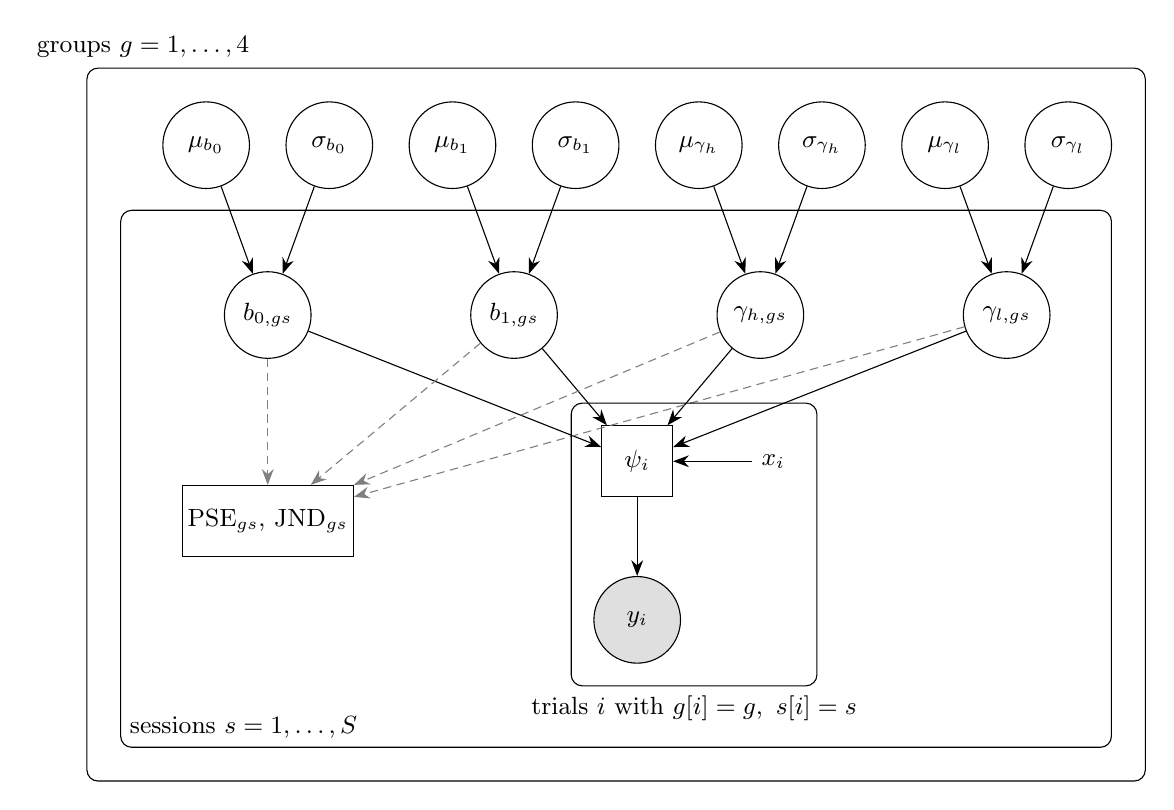
\begin{tikzpicture}[
    node distance=1.1cm and 0.45cm,
    latent/.style={circle, draw, minimum size=11mm, inner sep=0pt, font=\small},
    obs/.style={latent, fill=gray!25},
    det/.style={rectangle, draw, minimum size=9mm, inner sep=2pt, font=\small},
    const/.style={font=\small},
    arr/.style={-{Stealth[length=2mm]}},
    plate/.style={draw, rounded corners, inner sep=8pt}
  ]
  % hyperparameters
  \node[latent] (mub0) {$\mu_{b_0}$};
  \node[latent, right=of mub0] (sb0) {$\sigma_{b_0}$};
  \node[latent, right=of sb0] (mub1) {$\mu_{b_1}$};
  \node[latent, right=of mub1] (sb1) {$\sigma_{b_1}$};
  \node[latent, right=of sb1] (mugh) {$\mu_{\gamma_h}$};
  \node[latent, right=of mugh] (sgh) {$\sigma_{\gamma_h}$};
  \node[latent, right=of sgh] (mugl) {$\mu_{\gamma_l}$};
  \node[latent, right=of mugl] (sgl) {$\sigma_{\gamma_l}$};

  % session-level parameters
  \node[latent, below=1.6cm of $(mub0)!0.5!(sb0)$] (b0) {$b_{0,gs}$};
  \node[latent, below=1.6cm of $(mub1)!0.5!(sb1)$] (b1) {$b_{1,gs}$};
  \node[latent, below=1.6cm of $(mugh)!0.5!(sgh)$] (gh) {$\gamma_{h,gs}$};
  \node[latent, below=1.6cm of $(mugl)!0.5!(sgl)$] (gl) {$\gamma_{l,gs}$};

  % derived
  \node[det, below=1.6cm of b0] (pse) {PSE$_{gs}$, JND$_{gs}$};

  % trial level
  \node[det, below=1.4cm of $(b1)!0.5!(gh)$] (psi) {$\psi_i$};
  \node[obs, below=1.0cm of psi] (y) {$y_i$};
  \node[const, right=1.0cm of psi] (x) {$x_i$};

  \foreach \h/\p in {mub0/b0, sb0/b0, mub1/b1, sb1/b1, mugh/gh, sgh/gh, mugl/gl, sgl/gl}
    \draw[arr] (\h) -- (\p);
  \foreach \p in {b0, b1, gh, gl}
    \draw[arr] (\p) -- (psi);
  \foreach \p in {b0, b1, gh, gl}
    \draw[arr, densely dashed, gray] (\p) -- (pse);
  \draw[arr] (x) -- (psi);
  \draw[arr] (psi) -- (y);

  % plates
  \node[plate, fit=(x)(psi)(y), label={[font=\small]below:{trials $i$ with $g[i]=g,\ s[i]=s$}}] (ptrial) {};
  \node[plate, fit=(b0)(gl)(pse)(ptrial), inner sep=22pt,
        label={[font=\small, anchor=south west]south west:{sessions $s = 1,\dots,S$}}] (psess) {};
  \node[plate, fit=(mub0)(sgl)(psess), inner sep=12pt,
        label={[font=\small]above left:{groups $g = 1,\dots,4$}}] {};
\end{tikzpicture}
\end{center}

\noindent
Circles are random variables (shaded: observed), rectangles are deterministic
functions, and $x_i$ is a fixed covariate. Dashed arrows lead to derived
quantities that do not feed back into the likelihood.

%------------------------------------------------------------------------------
\section{Derived quantities: PSE and JND}

For each group and session the model records two summaries of the psychometric
curve.

\paragraph{Point of subjective equality (PSE):} the stimulus at which
$\psi = 1/2$. Solving
$\gamma_h + (1-\gamma_h-\gamma_l)\,\invlogit(b_0+b_1x) = \tfrac12$ gives
\[
  \text{PSE} = \frac{1}{b_1}\left[-b_0 + \log\frac{1-2\gamma_h}{1-2\gamma_l}\right].
\]

\paragraph{Just noticeable difference (JND):} half the stimulus distance between
the points where $\psi = 1/4$ and $\psi = 3/4$,
\[
  \text{JND} = \frac{x_{3/4} - x_{1/4}}{2}
  = \frac{1}{2b_1}\,\log\frac{(3-4\gamma_h)(3-4\gamma_l)}{(1-4\gamma_h)(1-4\gamma_l)} .
\]
Both are in units of the standardized stimulus. With
$\gamma_h=\gamma_l=0$ they reduce to $-b_0/b_1$ and $\log 3 / b_1$.

%------------------------------------------------------------------------------
\section{Implementation: non-centred parametrization}

To help the NUTS sampler, every distribution is written as a deterministic
transform of a standard variable, so the sampler only sees uniforms and
standard normals. With $g$ and $s$ indices suppressed:
\begin{align*}
  \mu_{b_0} &= -12 + 24\,u, & \mu_{b_1} &= 8\,u, & u &\sim \mathcal{U}[0,1], \\
  \sigma_{b_0} &= -12\,\log u, & \sigma_{b_1} &= -4\,\log u, & u &\sim \mathcal{U}[10^{-9},\,1-10^{-9}], \\
  \mu_{\gamma} &= z - 2.5, & \sigma_{\gamma} &= |1.25\,z|, & z &\sim \mathcal{N}(0,1), \\
  b_{k,gs} &= \sigma_{b_k,g}\, z + \mu_{b_k,g}, &
  \gamma_{\cdot,gs} &= 0.25\,\invlogit(\sigma_{\gamma,g}\, z + \mu_{\gamma,g}), &
  z &\sim \mathcal{N}(0,1).
\end{align*}
The bounds on $u$ for the exponentials avoid $\log 0$; they truncate the
distribution only negligibly. Each $u$ and $z$ is a separate variable.

\paragraph{Variables in the code.}
\begin{center}
\begin{tabular}{lll}
\toprule
PyMC variable & dims & meaning \\
\midrule
\code{u\_mu\_betas}, \code{mu\_betas} & (betas, groups) & $\mu_{b_0}$, $\mu_{b_1}$ \\
\code{u\_sig\_betas}, \code{sig\_betas} & (betas, groups) & $\sigma_{b_0}$, $\sigma_{b_1}$ \\
\code{z\_betas}, \code{beta\_vec} & (betas, groups, sessions) & $b_{0,gs}$, $b_{1,gs}$ \\
\code{z\_mu\_gams}, \code{mu\_gams} & (betas, groups) & $\mu_{\gamma_h}$ (index b0), $\mu_{\gamma_l}$ (index b1) \\
\code{z\_sig\_gams}, \code{sig\_gams} & (betas, groups) & $\sigma_{\gamma_h}$ (index b0), $\sigma_{\gamma_l}$ (index b1) \\
\code{z\_gams}, \code{gams} & (betas, groups, sessions) & $\gamma_{h,gs}$ (index b0), $\gamma_{l,gs}$ (index b1) \\
\code{gam\_h}, \code{gam\_l} & (groups, sessions) & $\gamma_{h,gs}$, $\gamma_{l,gs}$ \\
\code{PSE}, \code{JND} & (groups, sessions) & derived summaries \\
\code{resp} & (trials) & observed responses $y_i$ \\
\bottomrule
\end{tabular}
\end{center}
The lapse-rate variables reuse the \code{betas} dimension as a two-element axis:
its \code{b0} entry holds $\gamma_h$ and its \code{b1} entry holds $\gamma_l$.
The per-trial quantities ($b_0+b_1x_i$ and $\psi_i$) are computed as plain
tensors and not stored in the trace, to keep the trace small.

\paragraph{Size.} The sampler works on $32$ group-level standard variables
(8 per group) and $16S$ session-level ones (4 per group-session pair):
$32 + 16S$ in total, which is 704 for $S=42$.

\end{document}
